\section{Exercises on Shortest Path Problems}

\paragraph{}
\begin{quote}
The Services Department of GTC manages the relationships between the company and its customers. It handles all interactions with private customers ranging from new subscriptions and connections through maintenance and repair work. Recently, the company has launched the project Gold Service, which includes a 24 hours service. This means that if a customer reports a problem, then a technician makes a site call within 24 hours. Technicians move from one customer to another, and need not go back to the facility where the technician is stationed, except at the end of the working day. The calculation of shortest or fastest routes between two customer sites is not easy in practice, mainly because the circumstances in the road network change rapidly and regularly. Therefore, the company is testing a system which advises a technician about the route he has to take to the next customer, just after he has finished serving a customer.

The road map of the city is schematically depicted in Figure 1.10. There are 50 customer sites denoted by the dots, and labeled 1, ..., 50. A line denotes a direct road connection between two sites. Attached to each road is a number, denoting the distance between the connected sites in kilometers. For instance, the distance between site 22 and site 27 is 3.9 kilometers.
\end{quote}

\paragraph{}
We considered the graph with vertices corresponding to locations and edges corresponding to road segments. The weights of the edges correspond to length, time or cost, depending on the problem.

For finding shortest paths we used Floyd-Warshall algorithm for finding shortest path. For bigger graphs one might want to use Dijkstra’s algorithm instead. To find shortest path passing through certain edges, we tried all permutations and orientations of these edges and for each of them we concatenated shortest paths between consecutive edges (and paths from the start to the first edge and from the last edge to the end).

\subsection{Problem 1.1. Solution by Inspection and Computer}
\begin{quote}
It may be required to obtain a quick idea of distances between arbitrary pairs of sites, for instance if the computer system fails and the calculations need to be done by inspection. Suggest by inspection, as short a route as possible between the following pairs of sites. Do not use more than 20 seconds to determine each separate path.
\begin{enumerate}[(1)]
\item From site 8 to site 31.
\item From site 5 to site 38.
\item From site 1 to site 48.
\item From site 4 to site 41.
\item From site 24 to site 30.
\item From site 9 to site 47.
\end{enumerate}

Now use a computer program to calculate shortest routes (in kilometers) between the pairs of sites given above. It is normal that the computer calculations yield better results.
\end{quote}

\begin{figure}[H]
	\centering
	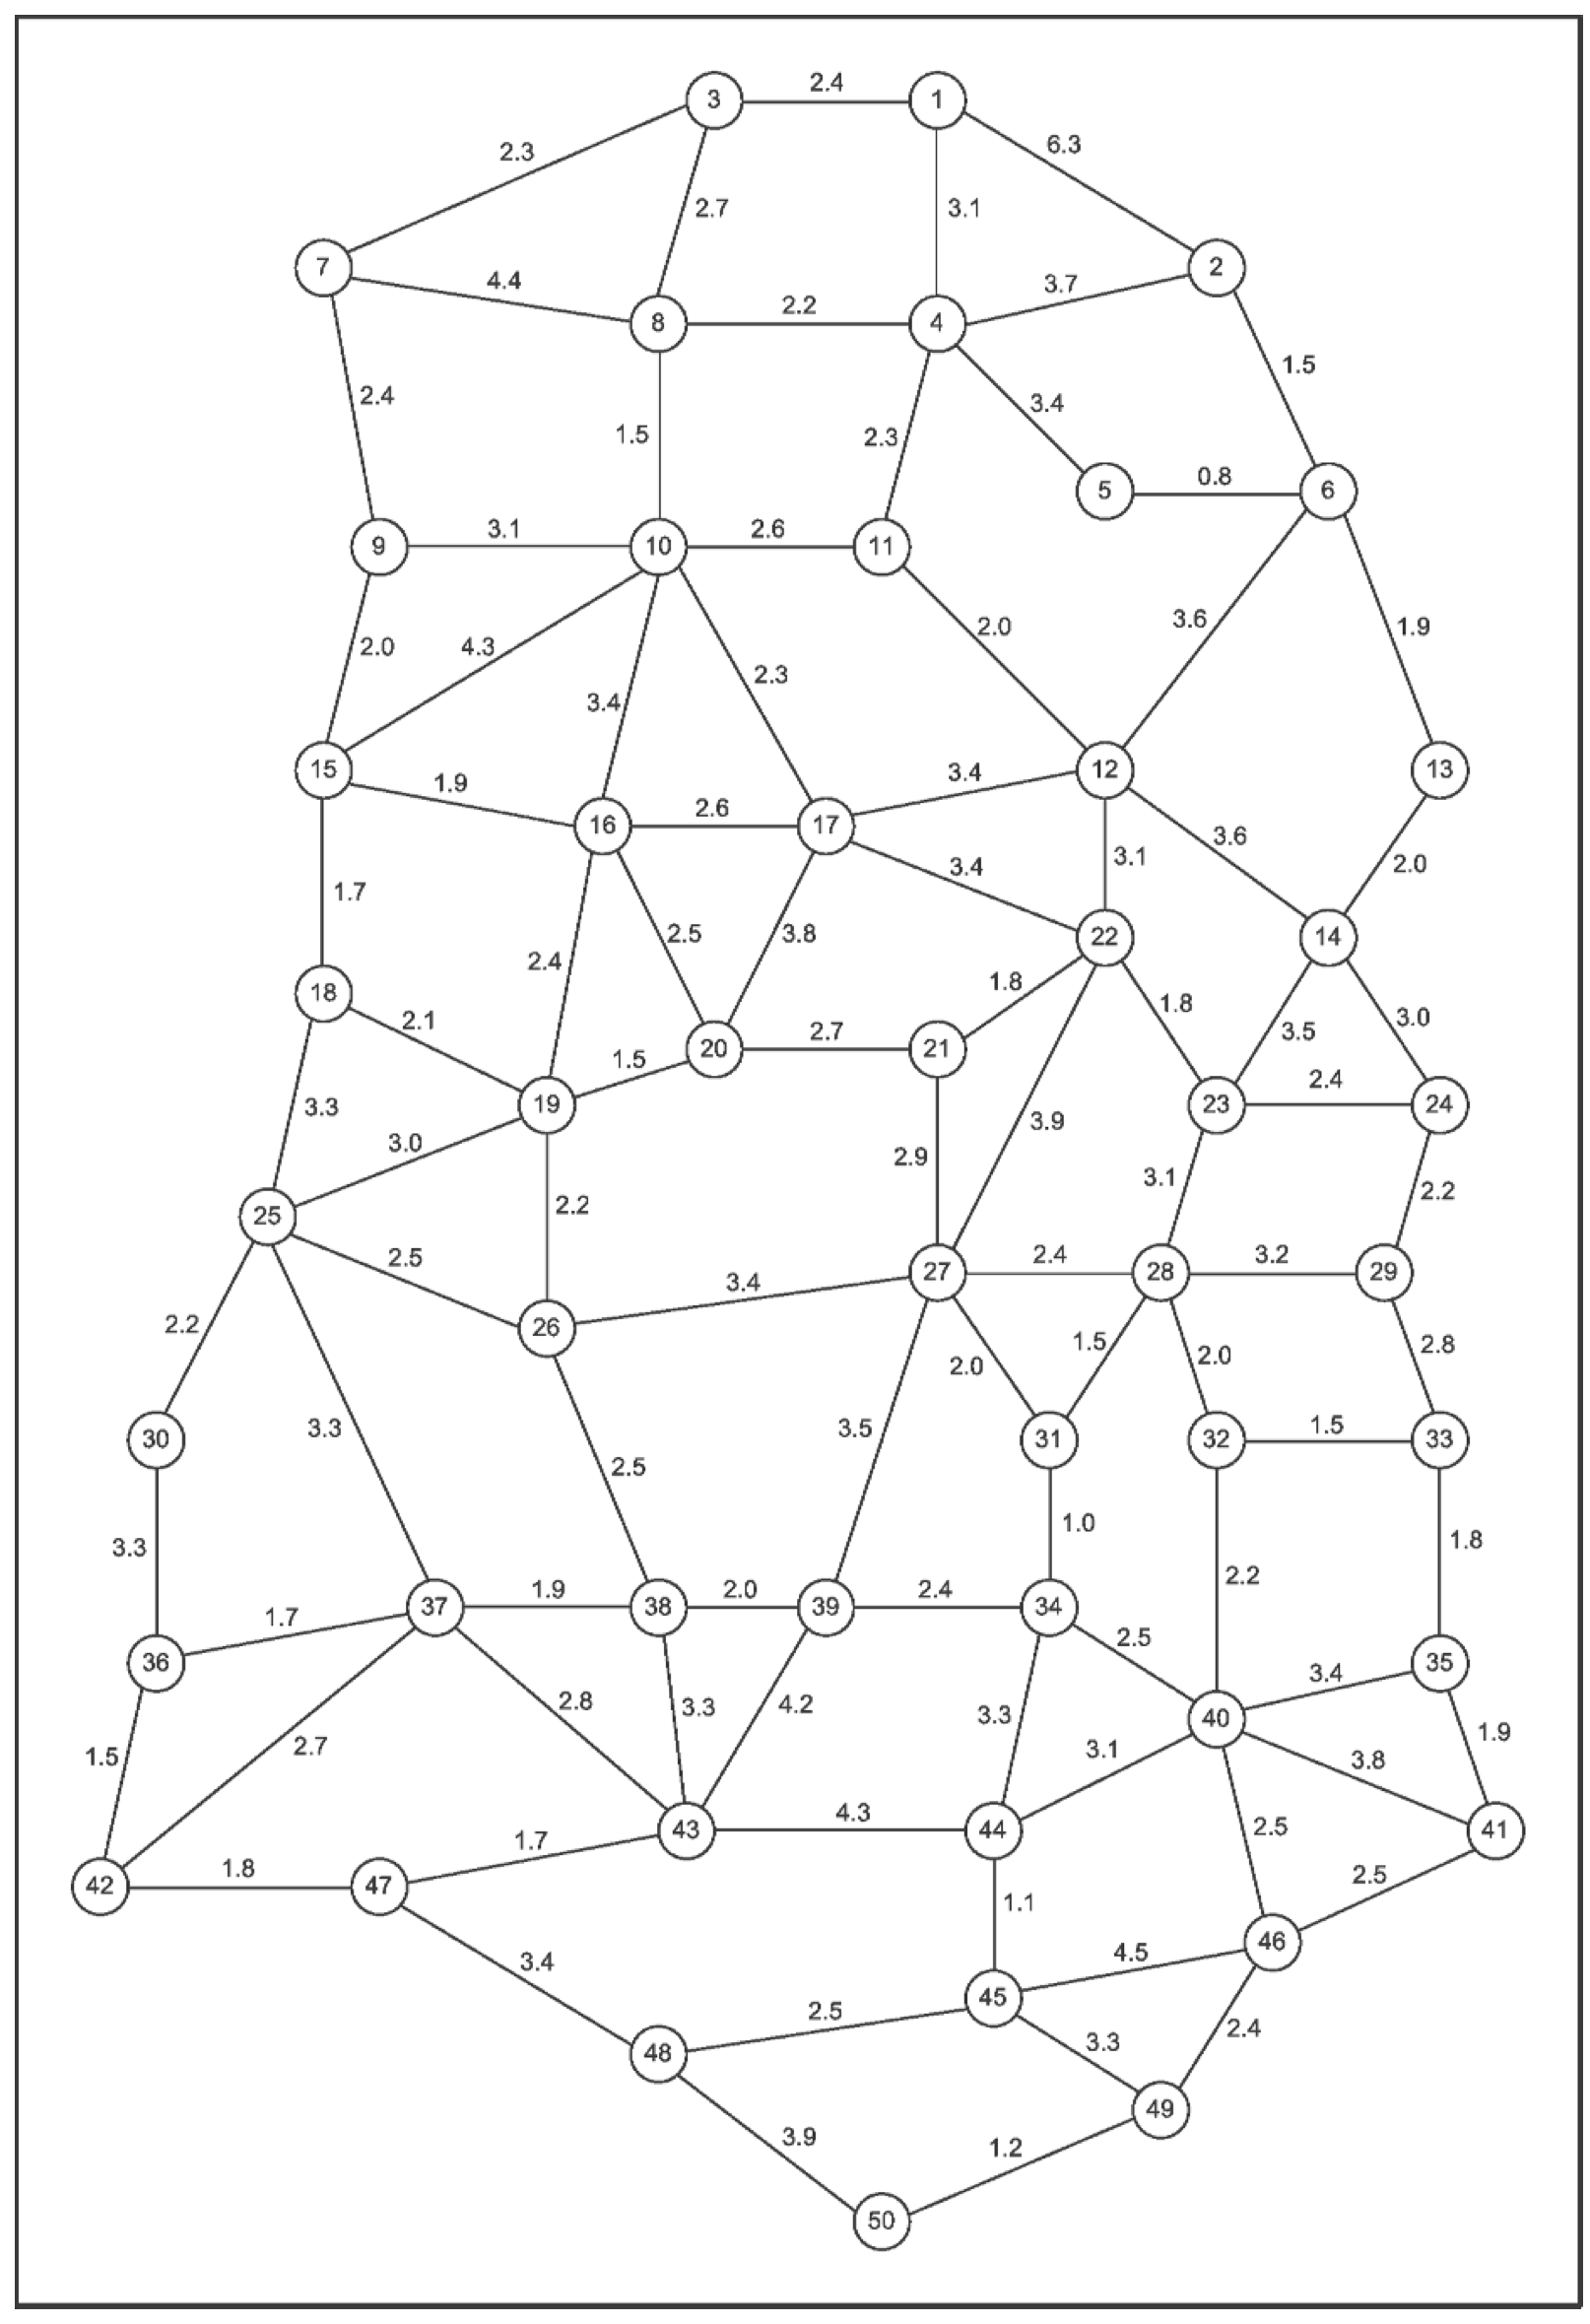
\includegraphics[scale=1]{./img/figure1-10.png}
	\caption{Schematic road map with distances in kilometers}
	\label{figure1-10}
\end{figure}

\paragraph{}
Let edge weights be equal to lengths in kilometers from figure \ref{figure1-10}. The paths found by hand and shortest paths are shown in table \ref{manual_vs_automatic_1_11}. Only one path is guessed correctly.

\begin{table}[H]
\centering
\begin{tabular}{|c|p{6cm}|c|c|p{6cm}|}
\hline
 & Path found manually in 20s & Len & Len & Path found automatically \\ \hline
(1) & $ 8 \rightarrow 10 \rightarrow 17 \rightarrow 22 \rightarrow 27 \rightarrow 31 $ & 13.1 & 13.1 & $ 8 \rightarrow 10 \rightarrow 17 \rightarrow 22 \rightarrow 27 \rightarrow 31 $ \\ \hline
(2) & $ 5 \rightarrow 6 \rightarrow 13 \rightarrow 14 \rightarrow 23 \rightarrow 28 \rightarrow 31 \rightarrow 34 \rightarrow 39 \rightarrow 38 $ & 18.2 & 16.9 & $ 5 \rightarrow 6 \rightarrow 12 \rightarrow 22 \rightarrow 27 \rightarrow 39 \rightarrow 38 $ \\ \hline
(3) & $ 1 \rightarrow 4 \rightarrow 11 \rightarrow 12 \rightarrow 22 \rightarrow 21 \rightarrow 27 \rightarrow 31 \rightarrow 34 \rightarrow 44 \rightarrow 45 \rightarrow 48 $ & 25.1 & 24.3 & $ 1 \rightarrow 4 \rightarrow 11 \rightarrow 12 \rightarrow 22 \rightarrow 27 \rightarrow 31 \rightarrow 34 \rightarrow 44 \rightarrow 45 \rightarrow 48 $ \\ \hline
(4) & $ 4 \rightarrow 11 \rightarrow 12 \rightarrow 14 \rightarrow 24 \rightarrow 29 \rightarrow 33 \rightarrow 35 \rightarrow 41 $ & 19.6 & 19.5 & $ 4 \rightarrow 11 \rightarrow 12 \rightarrow 22 \rightarrow 23 \rightarrow 28 \rightarrow 32 \rightarrow 33 \rightarrow 35 \rightarrow 41 $ \\ \hline
(5) & $ 24 \rightarrow 29 \rightarrow 28 \rightarrow 27 \rightarrow 26 \rightarrow 25 \rightarrow 30 $ & 15.9 & 15.4 & $ 24 \rightarrow 23 \rightarrow 22 \rightarrow 21 \rightarrow 20 \rightarrow 19 \rightarrow 25 \rightarrow 30 $ \\ \hline
(6) & $ 9 \rightarrow 15 \rightarrow 18 \rightarrow 19 \rightarrow 26 \rightarrow 38 \rightarrow 43 \rightarrow 47 $ & 15.5 & 14.8 & $ 9 \rightarrow 15 \rightarrow 18 \rightarrow 25 \rightarrow 37 \rightarrow 42 \rightarrow 47 $ \\ \hline
\end{tabular}
\caption{Shortest paths guessed by human and found by machine.}
\label{manual_vs_automatic_1_11}
\end{table}

\begin{quote}
In order to obtain an idea about the time required to go from one location to another, we can also make use of a road map in which the travel times are given for each connected pair of locations. We have depicted the schematic road map in Figure 1.11 with the travel times in minutes. Travel times are of course less precisely determined than distances, and may also change suddenly. These uncertainty aspects have to be taken into account when performing realistic calculations based on them.
\end{quote}

\subsection{Problem 1.2. What Happens If}

\paragraph{}
\begin{quote}
Use the time network depicted in Figure 1.11 to respond to the following. Unless specified each part is independent of the others.
\end{quote}

\begin{figure}[H]
\centering
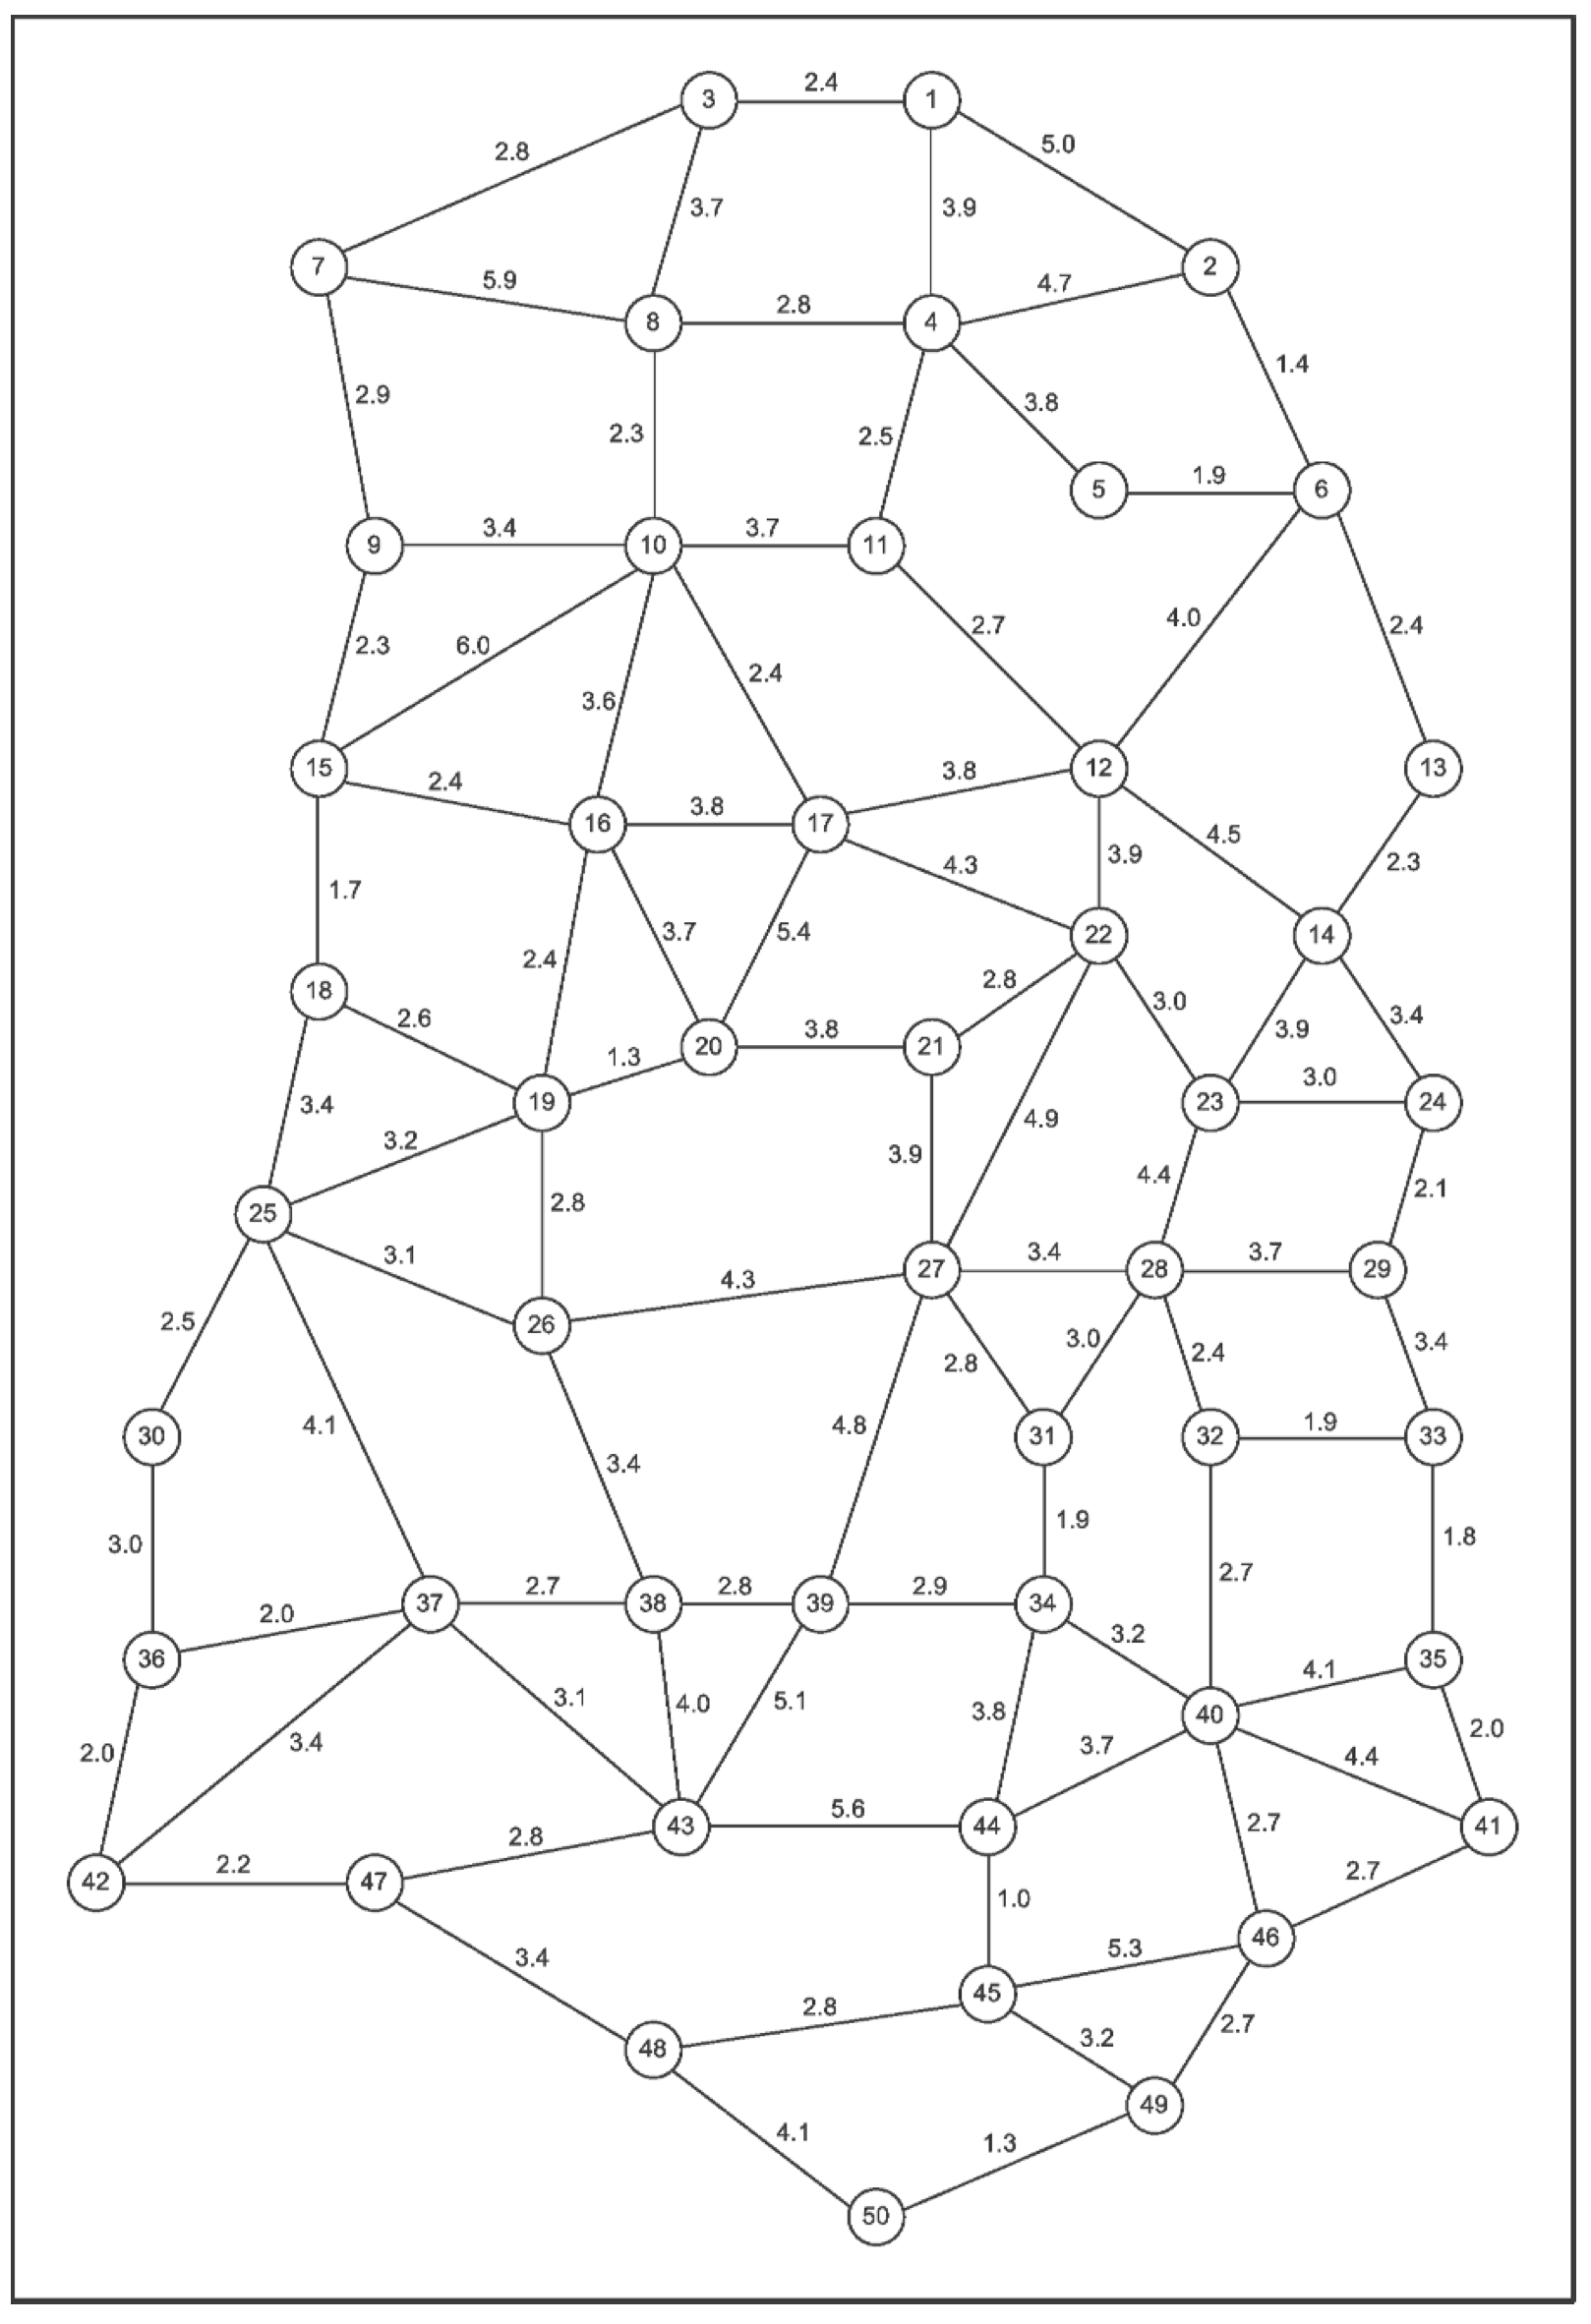
\includegraphics[scale=1]{./img/figure1-11.png}
\caption{Schematic road map with travel times in minutes}
\label{figure1-11}
\end{figure}

\paragraph{(a)}
\begin{quote}
Calculate quickest routes (in minutes) between the pairs of sites from Prob- lem 1.1.
\end{quote}

\paragraph{}
The routes are given in table \ref{quickest_routes_12}.

\begin{table}[H]
\centering
\begin{tabular}{|c|r|l|}
\hline
 & Path & Length \\ \hline
(1) & $ 8 \rightarrow 10 \rightarrow 17 \rightarrow 22 \rightarrow 27 \rightarrow 31 $ & 16.7 \\ \hline
(2) & $ 5 \rightarrow 4 \rightarrow 8 \rightarrow 10 \rightarrow 16 \rightarrow 19 \rightarrow 26 \rightarrow 38 $ & 21.1 \\ \hline
(3) & $ 1 \rightarrow 3 \rightarrow 7 \rightarrow 9 \rightarrow 15 \rightarrow 18 \rightarrow 25 \rightarrow 30 \rightarrow 36 \rightarrow 42 \rightarrow 47 \rightarrow 48 $ & 28.6 \\ \hline
(4) & $ 4 \rightarrow 11 \rightarrow 12 \rightarrow 14 \rightarrow 24 \rightarrow 29 \rightarrow 33 \rightarrow 35 \rightarrow 41 $ & 22.4 \\ \hline
(5) & $ 24 \rightarrow 29 \rightarrow 28 \rightarrow 27 \rightarrow 26 \rightarrow 25 \rightarrow 30 $ & 19.1 \\ \hline
(6) & $ 9 \rightarrow 15 \rightarrow 18 \rightarrow 25 \rightarrow 30 \rightarrow 36 \rightarrow 42 \rightarrow 47 $ & 17.1 \\ \hline
\end{tabular}
\caption{Quickest routes}
\label{quickest_routes_12}
\end{table}

\paragraph{(b)}
\begin{quote}
Determine for each of these quickest routes the range within which the travel time between the sites 8 and 10 may change without changing the calculated quickest route.
\end{quote}

\paragraph{}
For paths containing edge 8---10 the range is $[-\infty,2.3+u]$, where $u$ is the upper tolerance of edge 8---10 with respect to the path and $2.3$ is the weight of edge 8---10. In other words, we can increase the weight of an edge by no more than its upper tolerance without changing the shortest path.

\paragraph{}
For paths not containing edge 8---10 the range is $[2.3-l,+\infty]$, where $l$ is the lower tolerance of edge 8---10 with respect to the path and $2.3$ is the weight of edge 8---10. In other words, we can decrease the weight of an edge by less than its lower tolerance without changing the shortest path.

\paragraph{}
The sought-for ranges of weight of edge 8---10 for different paths:
\begin{enumerate}[(1)]
\item $ [-\infty, 5.2] $
\item $ [-\infty, 3.3] $
\item $ [0.2, +\infty] $
\item $ [-2.4, +\infty] $
\item $ [-7.6, +\infty] $
\item $ [-7.5, +\infty] $
\end{enumerate}

\paragraph{(c)}
\begin{quote}
What could be a plausible reason for the range in (b) in the case of Problem 1.1 pair (1) being much larger than the one for Problem 1.1 pair (2)?
\end{quote}

\paragraph{}
In case (2) we can do without the edge 8---10 just fine. The sequence $4 \rightarrow 8 \rightarrow 10$ can be replaced with $4 \rightarrow 11 \rightarrow 10$ adding only $1.1$ to path length (though the real shortest path without edge 8---10 takes completely different direction: $5 \rightarrow 6 \rightarrow 12 \rightarrow 17 \rightarrow 16 \rightarrow 19 \rightarrow 26 \rightarrow 38$).

\paragraph{}
In case (1) the path seems to rely stronger on edge 8---10. After removing it, the shortest path becomes $8 \rightarrow 4 \rightarrow 11 \rightarrow 12 \rightarrow 22 \rightarrow 27 \rightarrow 31$.

\paragraph{(d)}
\begin{quote}
Show, using tolerance intervals, that the shortest route in case of Problem 1.1 pair (6) is not unique. Calculate an alternative optimal solution. Answer the same questions for Problem 1.1 pair (3).
\end{quote}

\paragraph{}
The upper tolerance values for edges of path are given in tables \ref{tolerances-1-2d-6} and \ref{tolerances-1-2d-3} for cases (6) and (3) respectively. It can be seen that the minimum upper tolerance is zero, which means the shortest path is not unique. An alternative path can be found by removing any edge with zero upper tolerance. One of the  alternative paths for case (6) is $ 9 \rightarrow 15 \rightarrow 18 \rightarrow 25 \rightarrow 37 \rightarrow 42 \rightarrow 47 $. One of the alternative paths for case (3) is $ 1 \rightarrow 3 \rightarrow 7 \rightarrow 9 \rightarrow 15 \rightarrow 18 \rightarrow 25 \rightarrow 37 \rightarrow 42 \rightarrow 47 \rightarrow 48 $.

\begin{table}[H]
\centering
\begin{tabular}{|c|l|}
\hline
Edge & Upper Tolerance \\ \hline
9---15 & 52 \\ \hline
15---18 & 29 \\ \hline
18---25 & 24 \\ \hline
25---30 & 0 \\ \hline
30---36 & 0 \\ \hline
36---42 & 0 \\ \hline
42---47 & 3 \\ \hline
\end{tabular}
\caption{Upper tolerances in case (6)}
\label{tolerances-1-2d-6}
\end{table}

\begin{table}[H]
\centering
\begin{tabular}{|c|l|}
\hline
Edge & Upper Tolerance \\ \hline
1---3 & 16 \\ \hline
3---7 & 16 \\ \hline
7---9 & 16 \\ \hline
9---15 & 16 \\ \hline
15---18 & 16 \\ \hline
18---25 & 16 \\ \hline
25---30 & 0 \\ \hline
30---36 & 0 \\ \hline
36---42 & 0 \\ \hline
42---47 & 3 \\ \hline
47---48 & 16 \\ \hline
\end{tabular}
\caption{Upper tolerances in case (3)}
\label{tolerances-1-2d-3}
\end{table}

\paragraph{(e)}

\begin{quote}
Due to an accident, no traffic is possible between the sites 8 and 10. Show that the length of any shortest route that contains road segment 8 – 10 is changed as if the value of road segment 8 – 10 is pegged to its upper tolerance value with respect to that quickest route.
\end{quote}

\paragraph{}
Let's prove it. Let the value of segment 8---10 be $x$. Let its upper tolerance be $u$ (that is, the value can be increased to up to $x+u$ no shortest path passes through it). Let the length of shortest path between $A$ and $B$ be $s$.

Lemma 1. If we increase value of the edge by $z$ ($z \leq u$), the shortest path will have length $s+z$.

Proof. If we increase value of the edge by $z$ ($z \leq u$), at least one shortest path will pass through edge 8---10 (by definition of $u$). Such shortest path consists of three parts: path from $A$ to 8, edge 8---10, path from 10 to $B$. The first and third part must be optimal for the whole path to be optimal. Both optimal paths can't pass through edge 8---10 as it would introduce a cycle to the shortest path. So increasing weight of 8---10 doesn't affect these paths. So the weight of the path is only increased by $z$.

Lemma 2. Shortest path not including edge 8---10 is no shorter than $s+u$.

Proof. Assume the opposite. Let the shortest path without edge 8---10 have length $s+v$. Then for any $z$ ($z>v$, $z \leq u$) this path would be shorter than $s+z$ if we increase $x$ by $z$, which violates lemma 1.

Now suppose we increased the weight of 8---10 to $x+u+\varepsilon$. There exists a path from $A$ to $B$ passing through 8---10 with length $s+u+\varepsilon$ (see proof of lemma 1), but it's not optimal. This means the shortest path not passing through 8---10 is shorter than $s+u+\varepsilon$ for any positive $\varepsilon$. This, along with lemma 2, means that the shortest path not passing through edge 8---10 has length $s$. The theorem has been proved.

\paragraph{(f)}

\begin{quote}
Determine a second quickest route between 8 and 31 for the network in Figure 1.11. Show that the “length” (in minutes) of this route can also be determined by using tolerance intervals.
\end{quote}

\paragraph{}
The first quickest route is $ 8 \rightarrow 10 \rightarrow 17 \rightarrow 22 \rightarrow 27 \rightarrow 31 $ and has length 16.7. The second quickest route is $ 8 \rightarrow 10 \rightarrow 16 \rightarrow 19 \rightarrow 26 \rightarrow 27 \rightarrow 31 $ and has length 18.2. The difference between 18.2 and 16.7 should be equal to the minimum upper tolerance of edges of the first shortest path. These tolerances are given in table \ref{tolerances-1-2f}. The difference is indeed equal to minimum tolerance.

\begin{table}[H]
\centering
\begin{tabular}{|c|l|}
\hline
Edge & Upper Tolerance \\ \hline
8-10 & 2.9 \\ \hline
10-17 & 1.5 \\ \hline
17-22 & 1.5 \\ \hline
22-27 & 1.5 \\ \hline
27-31 & 2.7 \\ \hline
\end{tabular}
\caption{Upper tolerances}
\label{tolerances-1-2f}
\end{table}

\paragraph{(g)}

\begin{quote}
Quickest routes sometimes need to be determined in the presence of restrictions that certain roads of the network have to be included (or excluded) in the route. Such problems may occur when cable work activities are executed in certain streets and the work in process has to be checked. Determine quickest routes in the following situations.
\end{quote}

\begin{enumerate}[1.]
\item
\begin{quote}
From site 27 to site 16, including road segment 21 – 22.
\end{quote}

$ 27 \rightarrow 21 \rightarrow 22 \rightarrow 17 \rightarrow 16 $  (length 14.8)
\item
\begin{quote}
From site 35 to site 26, including road segment 31 – 34.
\end{quote}

$ 35 \rightarrow 40 \rightarrow 34 \rightarrow 31 \rightarrow 27 \rightarrow 26 $  (length 16.3)
\item
\begin{quote}
From site 39 to site 3, including road segment 16 – 17.
\end{quote}

$ 39 \rightarrow 38 \rightarrow 26 \rightarrow 19 \rightarrow 16 \rightarrow 17 \rightarrow 10 \rightarrow 8 \rightarrow 3 $  (length 23.6)
\item
\begin{quote}
From site 44 to site 14, including road segment 27 – 28.
\end{quote}

$ 44 \rightarrow 34 \rightarrow 31 \rightarrow 27 \rightarrow 28 \rightarrow 23 \rightarrow 14 $  (length 20.2)
\item
\begin{quote}
From site 15 to site 14, including road segments 16 – 10 and 12 – 22.
\end{quote}

$ 15 \rightarrow 16 \rightarrow 10 \rightarrow 17 \rightarrow 22 \rightarrow 12 \rightarrow 14 $  (length 21.1)
\item
\begin{quote}
From site 26 to site 48, including road segments 35 – 40 and 40 – 41. Deter-
mine a second best and a third quickest route as well.
\end{quote}

First quickest: $ 26 \rightarrow 27 \rightarrow 31 \rightarrow 34 \rightarrow 40 \rightarrow 35 \rightarrow 41 \rightarrow 40 \rightarrow 44 \rightarrow 45 \rightarrow 48 $  (length 30.2)

Second quickest: $ 26 \rightarrow 38 \rightarrow 39 \rightarrow 34 \rightarrow 40 \rightarrow 35 \rightarrow 41 \rightarrow 40 \rightarrow 44 \rightarrow 45 \rightarrow 48 $  (length 30.3)

Third quickest: $ 26 \rightarrow 27 \rightarrow 28 \rightarrow 32 \rightarrow 40 \rightarrow 35 \rightarrow 41 \rightarrow 40 \rightarrow 44 \rightarrow 45 \rightarrow 48 $  (length 30.8)

To find second quickest path we removed an edge from quickest path and found the shortest path. Among such paths we took the shortest. Similarly, to find the third shortest path we removed some edge from the first shortest path and some edge from the second shortest path, and found the shortest path in what remained. Among all $O(N^2)$ such shortest paths we again took the shortest.
\item
\begin{quote}
A driver goes from site 37 to site 43 and has to pass the road segments 35 – 40 and 40 – 41. Is this possible to do within 35 minutes?
\end{quote}

The quickest path is $ 37 \rightarrow 38 \rightarrow 39 \rightarrow 34 \rightarrow 40 \rightarrow 35 \rightarrow 41 \rightarrow 40 \rightarrow 44 \rightarrow 43 $. It takes 31.4 minutes, so the answer is yes.
\end{enumerate}

\subsection{Problem 1.3. Manpower Planning}

\paragraph{}
\begin{quote}
The management of GTC has decided to replace its old cable network. The Research \& Development (R\&D) department has been asked to design a new cable that has ten times more capacity than the old cable. The cable has to be developed within the next five years. In this period all the three activities, viz. actual research, testing, and evaluation, have to be carried out. These three activities will be exe- cuted simultaneously. The most expensive part of the project concerns wages and training of the research employees. The company has already employed a number of researchers, but during the five years extra researchers will be needed. These extra researchers need to undergo special training due to the specific character of the work. R\&D requires a lower number of researchers during the testing period than during the evaluation and research periods. It has decided to work with half-yearly planning periods because, in general, the nature of the work changes noticeably every half year. The company has to design a schedule of hiring and firing people. The next question is on determining an optimal hiring-firing schedule.

The numbers of extra research employees needed for the research and development of the new cable for the next ten consecutive half-year periods are listed in Table 1.1. The half-year periods are labeled 1, . . . , 10. The training of a new researcher requires an investment of \texteuro 8,000. Firing a person is expensive, it costs \texteuro 24,000 per fired person. Moreover, if there are fewer people under contract than required, it costs the company an average of \texteuro 32,000 per person per half-year.
\end{quote}

\begin{table}[H]
\centering
\begin{tabular}{lcccccccccc}
\hline
Period & 1 & 2 & 3 & 4 & 5 & 6 & 7 & 8 & 9 & 10 \\ \hline
Extra researchers & 9 & 7 & 6 & 12 & 11 & 8 & 13 & 11 & 7 & 10 \\ \hline
\end{tabular}
\caption{Extra researcher requirement for the project}
\label{extra-researchers}
\end{table}

\paragraph{}
Probably there is a typo in the sentence "Moreover, if there are fewer people under contract than required, it costs the company an average of €32,000 per person per half-year". "fewer" in that sentence makes little sense, we'll assume "greater" instead.

\paragraph{(a)}
\begin{quote}
Determine a hiring-firing schedule to minimize cost, such that the number of employed researchers is as high as possible during each period. Use a shortest path problem formulation for solving this problem. What is the total number of redundant researchers in your solution?
\end{quote}

\paragraph{}
We found the shortest path on the following graph. Let $v_{i, j}$ ($0 \leq i \leq 10$, $0 \leq j \leq 13$) be the vertex of the graph corresponding to a state after period $i$ with $j$ employees under contract. There are three types of edges. Edges $v_{i, j} \rightarrow v_{i, j+1}$ with weight $\text{\texteuro} 8000$ mean hiring an employee. Edges $v_{i, j+1} \rightarrow v_{i, j}$ with weight \texteuro 24000 mean firing an employee. Edges $v_{i, j} \rightarrow v_{i+1, j}$ with weight $\text{\texteuro} \cdot (32000 -\varepsilon) \cdot (j - A_{i+1})$ ($j \geq A_{i+1}$, $A_k$ - required number of researchers for period $k$), mean waiting half year. Subtracting $\varepsilon$ maximizes the total number of employees during all periods when the cost is equal.

\paragraph{}
The optimal number of researchers for each period is shown in table \ref{researchers-1-3a}. The minimum total cost is \texteuro 496000.

\begin{table}[H]
\centering
\begin{tabular}{lcccccccccc}
\hline
Period & 1 & 2 & 3 & 4 & 5 & 6 & 7 & 8 & 9 & 10 \\ \hline
Researchers & 9 & 7 & 7 & 12 & 11 & 11 & 13 & 11 & 10 & 10 \\ \hline
\end{tabular}
\caption{Researchers under contract for each period in optimal schedule.}
\label{researchers-1-3a}
\end{table}

\paragraph{(b)}
\begin{quote}
In the periods 3 and 6 the expected work pressure is lower than normal. Determine an optimal solution for which the number of researchers under contract is minimal during these periods.
\end{quote}

\paragraph{}
We'll use the same graph as in (a), but without edges $v_{i, j} \rightarrow v_{i+1, j}$ for $i \in \{2, 5\}$, $j > A_{i+1}$. The optimal number of researchers for each period is shown in table \ref{researchers-1-3b}. The minimum total cost is still \texteuro 496000.

\begin{table}[H]
\centering
\begin{tabular}{lcccccccccc}
\hline
Period & 1 & 2 & 3 & 4 & 5 & 6 & 7 & 8 & 9 & 10 \\ \hline
Researchers & 9 & 7 & 6 & 12 & 11 & 8 & 13 & 11 & 10 & 10 \\ \hline
\end{tabular}
\caption{Researchers under contract for each period in optimal schedule.}
\label{researchers-1-3b}
\end{table}

\subsection{Problem 1.4. Subsidizing Connections}

\begin{quote}
In order to test the new cable, the company has decided to connect the university, located at site 3 of the network of Figure 1.10, to the R\&D building of GTC, located at site 46, using its cable network.
The City Council desires that two clinics associated with the city hospital, which are located at sites 8 and 20, be connected by a high capacity cable. So it wants to find out how much subsidy to give to GTC such that it is profitable for GTC to connect the two sites 8 and 20 with the new cable.
The City Council has decided to subsidize the laying of cable on the paths 8 – 10 – 16 – 20 and 29 – 28 – 31 – 34. The cables on either of the two paths cannot be interrupted. In order to minimize the disruption to the traffic circulation, it has also decided that work on laying cable on the paths 8 – 10 – 16 – 20, 16 – 19 – 26 – 38 – 37 – 42, 29 – 28 – 31 – 34 – 39 – 27 – 22 – 12 – 6, and 48 – 45 – 44 – 40 – 32 – 33 has to be executed in the directions 8 $\rightarrow$ 10 $\rightarrow$ 16 $\rightarrow$ 20, 16 $\rightarrow$ 19 $\rightarrow$ 26 $\rightarrow$ 38 $\rightarrow$ 37 $\rightarrow$ 42, 29 $\rightarrow$ 28 $\rightarrow$ 31 $\rightarrow$ 34 $\rightarrow$ 39 $\rightarrow$ 27 $\rightarrow$ 22 $\rightarrow$ 12 $\rightarrow$ 6, and 48 $\rightarrow$ 45  $\rightarrow$ 44 $\rightarrow$ 40 $\rightarrow$ 32 $\rightarrow$ 33, respectively. Actually, the subsidy also yields some extra profit for GTC. The construction costs are a multiple of the distances from Figure 1.10, in \texteuro 1,000’s per km. The subsidies on road segment 8 $\rightarrow$ 10 is \texteuro 3,500, on road segment 29 $\rightarrow$ 28 is \texteuro 6,800, on road segment 10 $\rightarrow$ 16 is \texteuro 6,600, on road segment 28 $\rightarrow$ 31 is \texteuro 2,900, on road segment 16 $\rightarrow$ 20 is \texteuro 4,900, and on road segment 31 $\rightarrow$ 34 is \texteuro 2,200.
\end{quote}

\paragraph{(a)}
\begin{quote}
Is it true that the subsidy is high enough, i.e., is it profitable for GTC to connect the sites 3 and 46 via the subsidized paths?
\end{quote}

\paragraph{}
We took a bidirectional weighted graph from figure \ref{figure1-10} and multiplied edge weights by \texteuro 1,000. We replaced bidirectional edges with directional edges on paths 8 $\rightarrow$ 10 $\rightarrow$ 16 $\rightarrow$ 20, 16 $\rightarrow$ 19 $\rightarrow$ 26 $\rightarrow$ 38 $\rightarrow$ 37 $\rightarrow$ 42, 29 $\rightarrow$ 28 $\rightarrow$ 31 $\rightarrow$ 34 $\rightarrow$ 39 $\rightarrow$ 27 $\rightarrow$ 22 $\rightarrow$ 12 $\rightarrow$ 6, and 48 $\rightarrow$ 45  $\rightarrow$ 44 $\rightarrow$ 40 $\rightarrow$ 32 $\rightarrow$ 33. We subtracted subsidy values from subsidized paths. We then found the shortest path from vertex 3 to vertex 46.

\paragraph{}
The cheapest path is $ 3 \rightarrow 8 \rightarrow 10 \rightarrow 16 \rightarrow 20 \rightarrow 21 \rightarrow 22 \rightarrow 23 \rightarrow 24 \rightarrow 29 \rightarrow 28 \rightarrow 31 \rightarrow 34 \rightarrow 40 \rightarrow 46 $. It is profitable for GTC to use subsidized paths.

\paragraph{(b)}
\begin{quote}
Knowing that GTC is also considering a new cable between the sites 2 and 50, and having confidence in a positive effect of the subsidies stated above, the City Council has approved an extra subsidy on paths 45 – 44 – 40 – 32 and 27 – 22 – 12 – 6. The subsidy on road segment 40→32 is \texteuro 3,200, on road segment 12 $\rightarrow$ 6 is \texteuro 7,700, on road segment 44 $\rightarrow$ 40 is \texteuro 4,700, on road segment 22 $\rightarrow$ 12 is \texteuro 7,100, on road segment 45 $\rightarrow$ 44 is \texteuro 2,800, and on road segment 27 $\rightarrow$ 22 is \texteuro 6,900.

Explain why it is not possible to use a shortest path algorithm to decide on the profitability for GTC to lay the cable on the two paths.
\end{quote}

\paragraph{}
We can't use shortest path algorithm in a straightforward way because the graph has cycles of negative weight. One of such cycles is $8 \rightarrow 10 \rightarrow 16 \rightarrow 20 \rightarrow 21 \rightarrow 22 \rightarrow 12 \rightarrow 6 \rightarrow 5 \rightarrow 4 \rightarrow 8$.

\paragraph{(c)}
\begin{quote}
After a re-calculation the City Council has decided to decrease the subsidy on 29 – 28 from \texteuro 6,800 to \texteuro 5,500. Answer the same question as in part (b).
\end{quote}

\paragraph{}
The answer is the same: cycle $8 \rightarrow 10 \rightarrow 16 \rightarrow 20 \rightarrow 21 \rightarrow 22 \rightarrow 12 \rightarrow 6 \rightarrow 5 \rightarrow 4 \rightarrow 8$ still has negative cost \texteuro $-4800$.

\paragraph{(d)}
\begin{quote}
Determine a solution (need not be optimal) for the following situation. The sites 3 and 46, and the sites 2 and 50 need to be connected by a cable, one between 3 and 46, and one between 2 and 50. If the two cables connect two sites with subsidy, then the subsidy is given only once.
\end{quote}

\paragraph{}
As long as the answer doesn't have to be optimal, we can take two arbitrary paths, for example $3 \rightarrow 8 \rightarrow 10 \rightarrow 17 \rightarrow 22 \rightarrow 23 \rightarrow 28 \rightarrow 31 \rightarrow 34 \rightarrow 40 \rightarrow 46$ and $ 2 \rightarrow 6 \rightarrow 13 \rightarrow 14 \rightarrow 23 \rightarrow 28 \rightarrow 31 \rightarrow 34 \rightarrow 40 \rightarrow 46 \rightarrow 49 \rightarrow 50 $ with total cost \texteuro 36800.
